\section{Preliminary Results}
\label{sec:eval}

\begin{figure}
    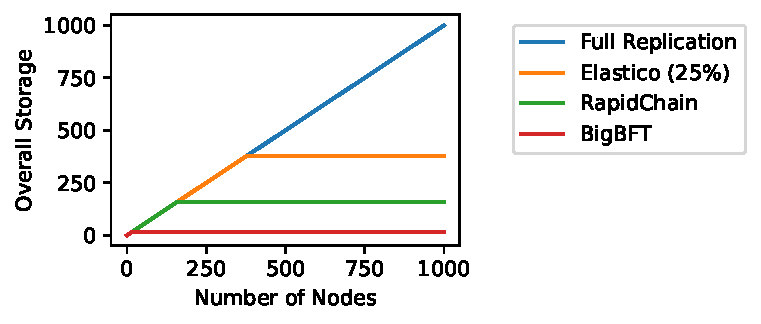
\includegraphics[width=0.95\linewidth]{graphs/redundancy}
    \caption{The overall storage consumption of various works, normalized to the state size.}
    \label{fig:redundancy}
\end{figure}

We perform numerical analysis to the overall storage consumption of different blockchains, and the result is shown in \autoref{fig:redundancy}.
The security parameters of \textsc{Elastico}, RapidChain and the active layer of \sys are the same $10^-6$.
Notice that \sys provides deterministic security guarantees.
Under this setting, \sys has the same probability of hitting fast path of the other works to ensure safety and liveness.
So this is a fair comparison since the performance of \sys's fast path is on par with the other works.
Also notice that \textsc{Elastico} is plotted with $\frac{1}{4}$ faulty nodes, which is the targeted scenario of its design.
As we discussed in \autoref{sec:bg}, its storage consumption will match full replication with $\frac{1}{3}$ faulty nodes.

The result shows that \sys achieves the best storage scalability.
\sys incurs storage overhead of at most $16\times$ state size regardless of the number of nodes.
RapidChain and \textsc{Elastico} can also achieve storage scalability but only with much larger upper bounds ($158\times$ and $378\times$ state size respectively).
This is because they have to pick committee sizes that are not smaller than these, so they can only start to shard at these scales.
And finally, full replication has unbounded storage consumption, growing linearly to the number of nodes.

\begin{figure}
    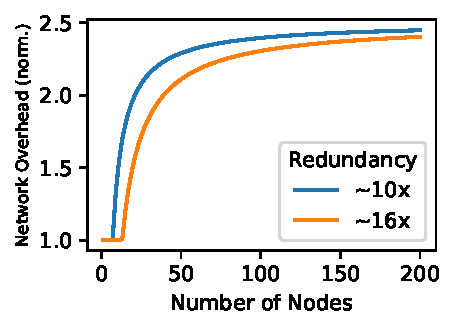
\includegraphics[width=0.6\linewidth]{graphs/network-overhead}
    \caption{The network traffic overhead brought by shard synchronization.
    The y-axis shows the total network traffic of \sys, normalized to baseline BFT protocols that only transmit transactions and replies.}
    \label{fig:network-overhead}
\end{figure}

We perform numerical analysis to project network traffic under a realistic setup.
In \autoref{fig:network-overhead} we show the result when \sys incurs $10\times$ and $16\times$ state size storage.
The exact plotting formula and parameter values are presented in appendix.
When the number of nodes is smaller than the targeted redundancy, every node effectively stores a full copy of the state and \sys has the same network traffic to the other BFT protocols.
As the number of nodes goes more than the redundancy rate, \sys starts to pay network traffic overhead for shard synchronization, but the overhead quickly converges to a constant amplifying factor to the baseline, and the network traffic of \sys never exceeds $2.5\times$ of the baseline traffic.
This is because all the BFT protocols have to disperse transactions and reply client the processing results anyway.
The network traffic of these activities increases linearly to the number of nodes, as well as the network traffic of shard synchronization.
Thus, our approach does not worsen the scalability of network communication.
